% HammerTime 100 final report — Overleaf source; compatible with Overleaf pdfLaTeX.
\documentclass[11pt,a4paper,oneside]{report}
\usepackage[a4paper,margin=1in,headheight=15pt,headsep=18pt,footskip=28pt]{geometry}
\usepackage[T1]{fontenc}\usepackage[utf8]{inputenc}\usepackage{newtxtext,newtxmath}\DeclareUnicodeCharacter{00B2}{\textsuperscript{2}}\DeclareUnicodeCharacter{00D7}{\ensuremath{\times}}\DeclareUnicodeCharacter{2019}{'}\DeclareUnicodeCharacter{2014}{---}
\usepackage{graphicx,booktabs,tabularx,longtable,array,float,caption,fancyhdr,setspace,enumitem}
\usepackage[hidelinks]{hyperref}\usepackage{titlesec}
\setstretch{1.04}\setlength{\parindent}{1.5em}\setlength{\parskip}{3pt}
\captionsetup{font=small,labelfont=bf,justification=centering}
\titleformat{\chapter}[display]{\normalfont\bfseries\centering}{\chaptertitlename\ \thechapter}{0pt}{\Large}
\titleformat{\section}{\normalfont\bfseries\large}{\thesection}{0.6em}{}
\titleformat{\subsection}{\normalfont\bfseries\normalsize}{\thesubsection}{0.6em}{}
\pagestyle{fancy}\fancyhf{}\fancyhead[L]{\small HammerTime -- Final Project Report}\fancyhead[R]{\small SCOPE -- VIT Chennai}\renewcommand{\headrulewidth}{0.4pt}\fancyfoot[C]{\thepage}
\graphicspath{{images/}}\begin{document}
\begin{titlepage}\centering\vspace*{1.1cm}{\large BCSE209L MACHINE LEARNING\\[0.4em] VELLORE INSTITUTE OF TECHNOLOGY CHENNAI\par}
\vspace{1.4cm}\rule{\textwidth}{0.6pt}\vspace{0.5cm}{\Huge\bfseries HammerTime 100\par}\vspace{0.35cm}{\Large Final Project Report\par}
\vspace{0.55cm}{\large A Dynamic Spatio Temporal Graph Neural Network for Formula 1 Traffic Delay Estimation\par}\vspace{0.45cm}{\normalsize Completed implementation and web application\par}
\vspace{0.45cm}{\normalsize Final case study: 2023 Monza Grand Prix\\Historical baseline: 2021 Abu Dhabi Grand Prix\par}\vspace{0.5cm}\rule{\textwidth}{0.6pt}\vfill
\begin{tabular}{@{}ll@{}}\textbf{A. Adithya Sai Pratheek} & 24BAI1445 \\
\textbf{M.S. Abhinav Sriram} & 24BAI1209\end{tabular}\par\vspace{1.4cm}School of Computer Science and Engineering\\VIT Chennai\par\vspace{0.4cm}24 October 2026\par\vspace{0.3cm}\href{https://github.com/andromeda7063/HammerTime}{github.com/andromeda7063/HammerTime}\par\vfill\end{titlepage}

We developed HammerTime to represent Formula 1 traffic as a changing graph and estimate a per-car mini-sector delay relative to a clean-air reference. Our final implementation extends the HammerTime50 prototype into a configurable data and machine learning pipeline, comparative evaluation, nine analytical visualizations, broadcast graphics, a Streamlit dashboard, and an interactive browser control room.

The system loads sessions through FastF1, aligns telemetry at 4 Hz, constructs directed leader-to-follower graphs, and forms history windows for a spatio-temporal graph attention network. We use nine node features, two graph attention layers, a temporal convolution, masked training, validation-based checkpoint selection, and isolated-car XGBoost and LSTM baselines. The configuration supports both chronological evaluation and race-held-out evaluation across multiple sessions.

Our final project submission includes the software implementation, saved checkpoint and history, presentation assets, test suite, application screenshots, and operating instructions. The available saved metrics report a test MAE of 0.046295 s and R² of -0.057059 over 983 target observations. The clean-air check passes in this summary; the complete-lap DRS check fails. These results do not establish the intended predictive accuracy or aerodynamic validity.

A central limitation is that the current target module constructs sector duration using nominal pace and prescribed wake penalties rather than measuring the counterfactual aerodynamic loss from observed sector timing. We therefore interpret the model as a research and demonstration implementation. We distinguish implementation completion from empirical validation, and identify the work required to support stronger scientific conclusions.

\subsection*{Project contributions}

\begin{itemize}[leftmargin=2em]\item An integrated M1 to M9 pipeline with session identity, graph masks, forecast windows, and training-only feature scaling.\end{itemize}

\begin{itemize}[leftmargin=2em]\item A graph attention and temporal convolution model with per-car regressions and comparable isolated-car baselines.\end{itemize}

\begin{itemize}[leftmargin=2em]\item An artifact-backed analysis dashboard and a separate interactive browser demonstration with track, telemetry, gallery, and broadcast views.\end{itemize}

\begin{itemize}[leftmargin=2em]\item A complete handover package covering source links, configuration, launch commands, screenshots, results, verification, and limitations.\end{itemize}

Keywords  Formula 1, traffic delay, graph attention, spatio temporal learning, FastF1, telemetry, machine learning, web application.

\clearpage

\clearpage\chapter*{Contents}\tableofcontents\clearpage\chapter*{List of Figures}\listoffigures\clearpage\chapter*{List of Tables}\listoftables\clearpage

Reading guide  Chapters 1 to 10 describe the research and implementation; Chapters 11 to 20 document the applications and visual outputs; Chapters 21 to 25 provide instructions, verification, and conclusions.

\clearpage

\clearpage\chapter*{1 Introduction and objectives}\addcontentsline{toc}{chapter}{1 Introduction and objectives}

\subsection*{Problem and motivation}

A car following another car experiences a changing traffic environment. Gap, tyre condition, driver pace, circuit position, and race interruptions all affect observed lap time. We designed HammerTime to model interactions between cars instead of treating each car as an independent time series. Our output is a delay estimate per driver and mini-sector; it is intended to support explanatory race graphics and research into traffic effects.

We define the intended learning problem as forecasting a sector delay y for each active car from a short sequence of graphs. A graph snapshot contains car features and directed proximity edges. The target concept is sector traversal time minus a comparable clean-air reference. This is an observational proxy: telemetry alone does not isolate the causal contribution of aerodynamic wake.

\subsection*{Objectives and scope}

\begin{itemize}[leftmargin=2em]\item Acquire and align session telemetry while preserving driver, lap, mini-sector, and race identity.\end{itemize}

\begin{itemize}[leftmargin=2em]\item Represent nearby leader-to-follower interactions and retain inactive driver slots through masks.\end{itemize}

\begin{itemize}[leftmargin=2em]\item Learn spatial and temporal patterns, evaluate against single-car baselines, and inspect physics-oriented checks.\end{itemize}

\begin{itemize}[leftmargin=2em]\item Present the work through reproducible command-line execution, dashboards, visualizations, and broadcast-style graphics.\end{itemize}

\subsection*{Technical background}

Graph attention networks aggregate neighbor information with learned attention coefficients [R8]. Spatio-temporal graph models combine relational structure with time-dependent observations, including in traffic forecasting [R9]. We adapt these ideas to moving cars: the adjacency changes with the time gap, and the prediction is a per-car regression rather than a fixed-road traffic count.

FastF1 supplies lap timing, telemetry, position, tyre, weather, and session information [R10]. PyTorch and PyTorch Geometric provide the neural model; pandas and NumPy support tabular processing; Streamlit, Plotly, Matplotlib, and browser canvas provide the presentation layer.

\subsection*{Requirements}

The implementation must preserve aligned time, avoid cross-race window mixing, mask invalid observations, fit feature scaling only on training inputs, and expose unavailable evaluation inputs. We treat the 2 s graph cutoff, 3 s clean-air threshold, and DRS loss band as configured modeling assumptions, not universal physical laws.

\clearpage

\clearpage\chapter*{2 Progress from HammerTime50}\addcontentsline{toc}{chapter}{2 Progress from HammerTime50}

Our HammerTime50 report established the first end-to-end prototype using the 2021 Abu Dhabi Grand Prix. We retain its problem formulation, graph interpretation, academic report structure, and emphasis on transparent results. The final project expands the implementation and adds the complete application and presentation layers. [R2]

\begin{center}\small\begin{tabularx}{\textwidth}{@{}>{\raggedright\arraybackslash}X>{\raggedright\arraybackslash}X>{\raggedright\arraybackslash}X@{}}

\toprule

Component & HammerTime50 baseline & HammerTime100 final implementation \\

\midrule

Session focus & 2021 Abu Dhabi R & 2023 Monza R default; multiple sessions supported \\

Node inputs & 4 normalized features & 9 features including five compound indicators \\

Spatial model & One custom message passing stage & Two multihead GATConv layers \\

Temporal model & Average pooling, W of 5 & Conv1d, W of 10, K of 5 \\

Evaluation & Chronological train and test & Train, validation, test; purge; optional race holdout \\

Baselines & No full final comparison suite & Isolated XGBoost and LSTM \\

Presentation & Graph and analytics images & V1 to V9, cards, Streamlit, browser control room \\

Verification & Midpoint checks and diagnosed faults & 26 defined unit tests and final verification record \\

\bottomrule\end{tabularx}\end{center}

\subsection*{Historical results and their interpretation}

The baseline records 416,879 aligned rows for 19 drivers, 21,941 graph snapshots, and 137,355 edges. It generated 5,483 windows in total: 4,112 training and 1,371 test windows. Its 3,393-parameter model reached MAE 1.1407 s and R² 0.2943 after ten epochs.

We do not use those values as a valid generalization benchmark. The midpoint report identifies a target lookup keyed only by driver and mini-sector, which overwrote lap-specific values. It also identifies unfiltered Safety Car data, quantized labels, and clipping. The reported 9,804 DRS-train time-step events are repeated detections across time, not 9,804 distinct trains.

The final implementation introduces lap-aware timestamp matching, session-scoped references, validity and Safety Car filters, split purging, and training-only scaling. These changes improve the software contracts. The current constructed target definition remains a separate scientific limitation, discussed in Chapter 5.

\clearpage

\clearpage\chapter*{3 End to end system architecture}\addcontentsline{toc}{chapter}{3 End to end system architecture}

We organize the implementation as nine modules controlled by run\_pipeline.py and configs/default.yaml. We process each configured session separately before combining compatible graph snapshots and labels for dataset construction. Presentation outputs follow evaluation. [R3, R4]

\captionof{table}{Scope comparison between the midpoint baseline and final implementation.}

\begin{center}\small\begin{tabularx}{\textwidth}{@{}>{\raggedright\arraybackslash}X>{\raggedright\arraybackslash}X>{\raggedright\arraybackslash}X@{}}

\toprule

Module & Source file & Responsibility \\

\midrule

M1 & src/ingest.py & Load FastF1 session and cache; export raw laps and telemetry. \\

M2 & src/preprocess.py & Align time, interpolate supported gaps, derive validity, pit and Safety Car flags, and car-ahead gaps. \\

M3 & src/target.py & Construct sector duration and clean-air reference; write per-session target rows. \\

M4 & src/graph.py & Create fixed-slot graph snapshots with node masks and directed RBF edges. \\

M5 & src/dataset.py & Match targets, form contiguous windows, split, purge overlap, and fit feature scaler. \\

M6 & src/model.py & Define projection, two GAT layers, temporal convolution, and regression head. \\

M7 & src/train.py & Train masked L1 model; early stopping, validation, history, and checkpoint. \\

M8 & src/evaluate.py & Held-out scores, physics checks, prediction records, and evaluation JSON. \\

M9 & src/baselines.py & Fit and score isolated-car XGBoost and LSTM comparisons. \\

\bottomrule\end{tabularx}\end{center}

\subsection*{Application and artifact flow}

FastF1 -> aligned telemetry -> targets + graphs       -> windows + purged splits -> scaler + ST-GNN       -> held-out evaluation + baselines -> JSON       -> visuals + broadcast cards -> StreamlitParquet + evaluation JSON -> optional JSON exporter                         -> static browser frontend

The Streamlit application consumes pipeline artifacts. The browser application uses exported summary data alongside a simulated track and demonstration charts. We do not provide an online inference API or a continuous race-feed service in this version.

\clearpage

\clearpage\chapter*{4 Data ingestion and preprocessing}\addcontentsline{toc}{chapter}{4 Data ingestion and preprocessing}

\subsection*{Session acquisition and storage}

We request the configured FastF1 session with lap, telemetry, and weather loading enabled. The default session is the 2023 Monza race. Each RaceId has its own cache and processed directory, preserving provenance when timestamps repeat across sessions. Ingestion raises an error if the requested source session cannot load; it does not replace unavailable race input with generated telemetry. [R3, R4]

\subsection*{Alignment and validity}

We resample each driver onto a shared 4 Hz grid with a 0.25 s step. Numeric channels are interpolated only where source support satisfies the configured maximum gap of 1.0 s. Unsupported data remains invalid. We preserve driver identity, lap number, compound, tyre life, distance, and available coordinates. Pit-lap and Safety Car flags support downstream filtering. Track status containing codes 4, 5, or 6 is flagged by the current implementation.

We divide the configured circuit length into 20 mini-sectors. The Monza default is 5,793 m, giving 289.65 m per equal-distance segment. Race order and within-lap distance support the nearest-car-ahead lookup and the gap field DeltaT. These derived gaps are model inputs and proximity indicators; they are not direct measurements of aerodynamic force.

\captionof{table}{Pipeline modules and their primary responsibilities.}

\begin{center}\small\begin{tabularx}{\textwidth}{@{}>{\raggedright\arraybackslash}X>{\raggedright\arraybackslash}X>{\raggedright\arraybackslash}X@{}}

\toprule

Field group & Representative columns & Use \\

\midrule

Identity & RaceId, Driver, Team & Join within the correct session and car. \\

Time and track & TimeSec, LapNumber, Distance, MiniSector & Alignment, windows, sector grouping and replay. \\

Telemetry & Speed, Throttle, Compound, TyreLife & Raw node feature construction. \\

Traffic & DriverAhead, DeltaT & Directed leader-to-follower topology. \\

Quality & IsValid, IsPitLap, IsSafetyCar & Mask nodes and reject contaminated windows. \\

Position & X, Y when available & Observed track views; unavailable coordinates prevent a measured map. \\

\bottomrule\end{tabularx}\end{center}

\subsection*{Data coverage in the submitted assets}

Our checked-in browser telemetry JSON contains 6,260 sampled records for 20 drivers and a 2023-Monza-R identifier. Driver summaries extend to lap 17. This sampled export is not a complete 53-lap archive. The original raw and aligned Parquet tables and the canonical evaluation report are not packaged in the current repository snapshot; a full rerun regenerates them.

\clearpage

\clearpage\chapter*{5 Target definition and clean air reference}\addcontentsline{toc}{chapter}{5 Target definition and clean air reference}

\subsection*{Intended prediction quantity}

Our intended target is the difference between the time required to traverse a mini-sector and a comparable clean-air reference for the same context. A positive value represents slower traversal; a negative value may represent faster traversal. Clean-air reference samples require an average car-ahead gap greater than 3 s and at least three qualifying samples for a reference group.

\begin{quote}\small\ttfamily sector delay = sector duration - clean air reference\par reference fallback = driver -> teammate -> session grid\par output clipping = [-2.0 s, 10.0 s]\end{quote}

\subsection*{Current implemented duration construction}

In the final source, calculate\_mini\_sector\_durations does not derive duration from observed entry and exit timestamps. We construct a nominal sector time of 3.50 + 0.40 × sin(0.75 × sector index) seconds, add a small driver offset, and add a prescribed traffic adjustment. Driver and lap offsets use Python hash values. The telemetry supplies grouping, timestamps, compound, and average gap. [R4]

\captionof{table}{Aligned telemetry fields used by processing, modeling, and presentation.}

\begin{center}\small\begin{tabularx}{\textwidth}{@{}>{\raggedright\arraybackslash}X>{\raggedright\arraybackslash}X>{\raggedright\arraybackslash}X@{}}

\toprule

Gap regime & Corner sector adjustment & Straight sector adjustment \\

\midrule

Below 0.8 s & 0.065 × wake + lap jitter & -0.012 × wake + lap jitter \\

0.8 s to 3.0 s & 0.030 × wake + lap jitter & -0.006 × wake + lap jitter \\

Greater than 3.0 s & Lap jitter & Lap jitter \\

\bottomrule\end{tabularx}\end{center}

Here wake = exp(-gap² / 2). The corner-sector set is hand-selected for Monza. We calculate clean-air medians within each RaceId, compound, and sector, resolving driver, teammate, then grid references. We omit rows without a supported reference and exclude invalid, pit, and Safety Car observations.

\subsection*{Scientific interpretation}

The resulting labels encode a designed traffic rule. A good score against them measures agreement with that construction; it does not validate measured aerodynamic loss. The Monza-specific sector assumptions also limit cross-circuit transfer. Hash-based offsets can change across Python processes unless hash seeding is controlled. We identify measured boundary-crossing durations, context-controlled references, and independent race validation as the main next research steps.

\clearpage

\clearpage\chapter*{6 Dynamic graph construction}\addcontentsline{toc}{chapter}{6 Dynamic graph construction}

At each aligned timestamp we keep 20 driver slots. Each active node contains speed, throttle, five tyre-compound indicators, tyre age, and mini-sector index. Inactive, pit, and invalid nodes remain masked. RaceId and the slot-to-driver mapping travel with each snapshot so target alignment does not depend on an accidental row order. [R4]

\begin{quote}\small\ttfamily Edge direction: leading car j -> following car i\par Create edge when 0 < gap(i,j) <= 2.0 seconds\par Edge weight = exp(-gap(i,j)^2 / (2 × sigma^2))\par Default sigma = 1.0 second\end{quote}

For illustration, gaps of 0.5 s, 1.0 s, and 2.0 s produce weights of approximately 0.8825, 0.6065, and 0.1353. These are proximity weights used as edge features by attention layers. They are not calibrated wake-force measurements. Our graph connects nearby leaders and followers; it is not a fully connected 20-car graph.

\begin{figure}[H]\centering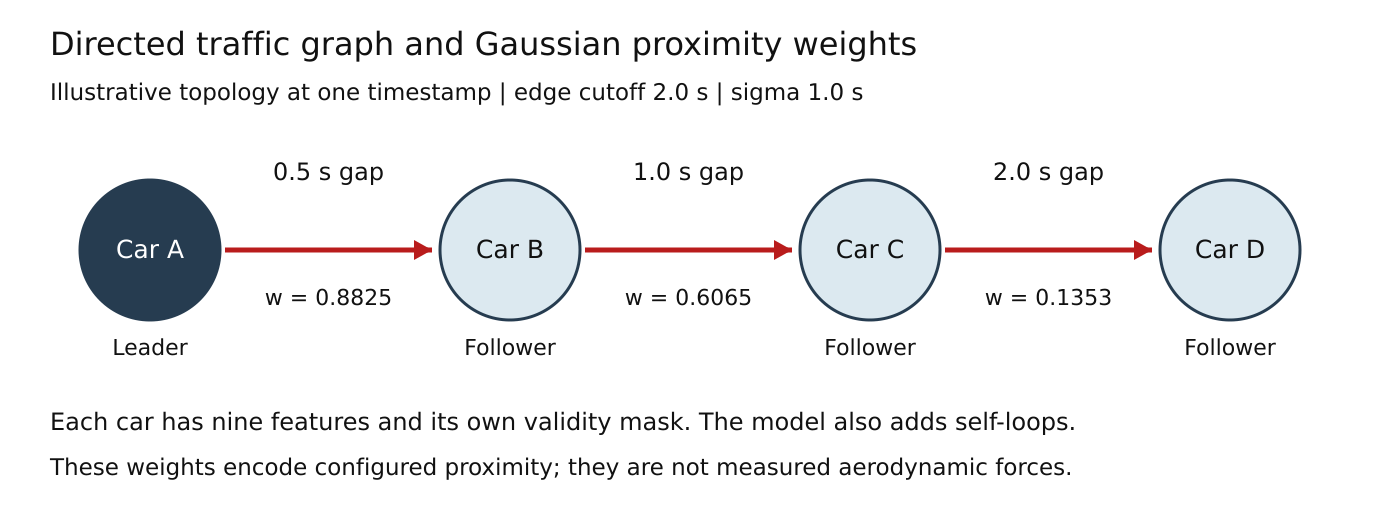
\includegraphics[width=0.88\textwidth,height=0.62\textheight,keepaspectratio]{figure_01.png}

\caption{Illustrative leader-to-follower topology showing how our configured RBF weights decrease with gap. This schematic explains the graph rule and does not represent an observed race snapshot.}

\end{figure}

The model adds explicit self-loops so a car can retain its own feature signal when no nearby-car edge exists. Two spatial layers allow information to propagate across successive links in a traffic chain. The visualization runner also contains a Monza fallback drawing, so the existence of V1 alone does not establish telemetry-backed coordinates.

\clearpage

\clearpage\chapter*{7 Spatio temporal graph neural network}\addcontentsline{toc}{chapter}{7 Spatio temporal graph neural network}

\subsection*{Neural architecture}

We implement HammerTimeSTGNN in PyTorch with PyTorch Geometric GATConv. A linear layer projects each nine-dimensional node vector to 64 hidden channels. Each of two attention layers has four heads with 16 channels per head, a scalar edge feature, ReLU activation, and dropout. Explicit self-loops carry unit edge attributes. [R4]

\begin{quote}\small\ttfamily Input window: W × N × 9\par Linear projection: W × N × 64\par GATConv layer 1: four heads, edge_dim 1\par GATConv layer 2: four heads, edge_dim 1\par Stack per-car history: N × 64 × W\par Temporal Conv1d: kernel 3, padded\par Select last temporal step: N × 64\par MLP regression head: N × 1\end{quote}

Our ten-snapshot history corresponds to ten 0.25 s sampling intervals, with 2.25 s between the first and final input timestamps. The five-snapshot forecast horizon is 1.25 s after the final input. We produce one delay scalar per driver at the forecast target, rather than five separate future predictions. Temporal convolution only receives the input history, so it does not inspect target-time observations.

\subsection*{Training procedure}

We minimize mean absolute error over valid target nodes. The mask has the same shape as predictions and targets. A batch without valid targets raises an error, and non-finite loss is rejected. Adam uses learning rate 0.001 and weight decay 0.0001. The default batch size is 128, dropout is 0.1, maximum training duration is 25 epochs, and early-stopping patience is six epochs.

We select the best validation checkpoint rather than the final epoch. The training code stores model weights, optimizer information, configuration, and the fitted feature scaler. The runner can reuse an existing checkpoint; the retraining option forces a new training run. We seed model and dataset operations with 42, while recognizing that the hash-derived target offsets need separate reproducibility control.

\subsection*{Implementation tradeoff}

The current batch forward method processes each graph window in a Python loop and stacks predictions. This is simple to inspect but is not a demonstrated low-latency serving design. We make no throughput or real-time latency claim without profiling on a declared device and workload.

\clearpage

\clearpage\chapter*{8 Experimental design and baseline models}\addcontentsline{toc}{chapter}{8 Experimental design and baseline models}

\subsection*{Window construction and leakage controls}

We match target timestamps to graph frames with a 0.1275 s tolerance and require contiguous windows with a 0.05 s continuity tolerance. Each sample needs at least one valid target. We reject Safety Car contamination across the history and forecast span, preserve driver-slot mapping, and prevent windows from crossing RaceId boundaries. [R4]

The default chronological split uses nominal ratios of 70 percent training, 15 percent validation, and 15 percent test. We purge overlap around split boundaries using the history and horizon settings. Exact retained counts depend on source coverage and filtering. StandardScaler is fitted using active training frames and then applied to validation and test inputs.

For stronger transfer evaluation we support a race-held-out split with at least three distinct RaceIds. Session-scoped clean-air references keep circuit timings separate. They do not by themselves establish prospective evaluation: references estimated using the full held-out session can incorporate information unavailable at forecast time. A future deployment evaluation should specify when reference samples become available.

\subsection*{Comparative models}

\captionof{table}{Hand-authored traffic adjustment in the current target builder.}

\begin{center}\small\begin{tabularx}{\textwidth}{@{}>{\raggedright\arraybackslash}X>{\raggedright\arraybackslash}X>{\raggedright\arraybackslash}X@{}}

\toprule

Model & Input and structure & Default training configuration \\

\midrule

ST-GNN & Multi-car graphs with nine features per node; two GAT layers and temporal Conv1d. & 64 hidden channels; 4 heads; 25 epochs maximum; batch 128. \\

XGBoost & One car only; flattened 10 × 9 feature history; no neighbors or edges. & 100 trees; depth 6; learning rate 0.05; subsample 0.8. \\

LSTM & One car only; temporal sequence of nine features; no neighbors or edges. & 64 hidden units; 2 layers; dropout 0.1; 40 epochs; batch 64. \\

\bottomrule\end{tabularx}\end{center}

We use the same partitioning and active target selection for the comparisons. The baseline isolation contract prevents another car’s features from entering the single-car models. MAE measures average absolute error in seconds; R² compares squared error with a constant-mean reference. A small MAE can coexist with a negative R² when predictions explain little target variation.

\clearpage

\clearpage\chapter*{9 Saved results and training history}\addcontentsline{toc}{chapter}{9 Saved results and training history}

Our repository includes a saved metric summary in frontend/data/metrics.json with source set to pipeline. We report its values below as saved results. It contains 983 target observations but not the prediction records or split metadata required to independently recompute the scores. The canonical evaluation\_report.json and source Parquet artifacts must accompany a reproducible run. [R5]

\captionof{table}{Model inputs and default comparison settings.}

\begin{center}\small\begin{tabularx}{\textwidth}{@{}>{\raggedright\arraybackslash}X>{\raggedright\arraybackslash}X>{\raggedright\arraybackslash}X@{}}

\toprule

Model & MAE in seconds & R squared \\

\midrule

HammerTime ST-GNN & 0.046294644 & -0.057058828 \\

Isolated temporal LSTM & 0.046343371 & -0.057039857 \\

Isolated XGBoost & 0.066571377 & -0.012636900 \\

\bottomrule\end{tabularx}\end{center}

The ST-GNN has the lowest saved MAE, but its advantage over LSTM is only about 0.000049 s, or 0.105 percent. Its MAE is approximately 30.46 percent lower than XGBoost. These arithmetic comparisons do not establish statistical significance or causal value from graph structure. Every saved R² is negative; we cannot claim that the intended explained-variance target has been achieved.

\subsection*{Acceptance criteria}

\captionof{table}{Values recorded in the checked-in metrics JSON summary.}

\begin{center}\small\begin{tabularx}{\textwidth}{@{}>{\raggedright\arraybackslash}X>{\raggedright\arraybackslash}X>{\raggedright\arraybackslash}X@{}}

\toprule

Criterion & Configured target & Saved outcome \\

\midrule

Held-out MAE & Less than 0.150 s & Pass in JSON summary \\

Held-out R² & 0.68 to 0.82 & Fail; -0.057059 \\

Clean-air prediction & Mean absolute penalty at most 0.050 s & Pass in JSON summary \\

Complete-lap DRS penalty & 0.40 to 0.80 s & Fail in JSON summary \\

\bottomrule\end{tabularx}\end{center}

\subsection*{Stored training history}

training\_history.csv contains 14 epochs. Training loss decreases from 0.0203611 s at epoch 1 to 0.0142894 s at epoch 14. The lowest validation MAE is 0.0168643 s at epoch 8; epoch 14 validation MAE is 0.0220497 s. These are validation values, not held-out test scores. The CSV does not encode its session, data version, or split, so we do not merge it with the JSON summary as one confirmed experiment.

The historical HammerTime50 scores describe a different session, target implementation, and faulty lookup. A direct numerical before-and-after accuracy claim would therefore be misleading.

\clearpage

\clearpage\chapter*{10 Physics checks and result provenance}\addcontentsline{toc}{chapter}{10 Physics checks and result provenance}

\subsection*{Clean air check}

We check whether the mean absolute predicted penalty for held-out observations with a gap greater than 3 s is at most 0.050 s. The saved JSON reports approximately 0.00001019 s over 245 observations and marks the check as passed. This tests near-zero behavior under our chosen definition; it is not evidence that physical wake effects vanish at exactly 3 s.

\subsection*{DRS train check}

We aggregate predicted penalties only for complete driver laps containing all configured mini-sectors. The strict proximity condition is 0 < gap < 0.8 s. The configured acceptance band is +0.40 to +0.80 s per lap. The saved summary reports -0.000203875 s per lap over ten complete laps, with a sector-level value near -0.00001019 s. The DRS check fails. [R5]

\subsection*{Why both score and physics checks matter}

A prediction close to zero can score well when the target distribution is concentrated near zero, while failing to reproduce traffic-related variation or cumulative lap loss. Our negative R² and failed DRS check prevent us from treating the low MAE as sufficient validation. The hand-set target construction further limits interpretation; agreement with its imposed shape cannot independently validate that shape.

\subsection*{Artifact consistency}

The saved PNGs, history CSV, checkpoint, frontend JSON, and static interface text are not a single documented run bundle. For example, the V2 graphic displays a different MAE and R² from metrics.json, and the V6 graphic displays different physics values. We retain the graphics as delivered presentation outputs and label them accordingly in Chapters 16 to 19.

Our static frontend also replaces a non-positive R² with a positive fallback and contains fixed pass messages. We therefore use the numeric JSON summary for the result table, not the dashboard’s decorative status text. Before any validated deployment, every score, pass indicator, card, and figure should be bound to the same versioned evaluation artifact.

\subsection*{Reproducible result bundle}

A complete experiment archive should contain the exact Git revision, dependency lock, configuration, session identifiers, processed data, target rows, split boundaries, scaler, checkpoint, prediction records, evaluation JSON, execution log, and generated figures. This allows results to be recomputed and ensures that presentation assets correspond to the declared experiment.

\clearpage

\clearpage\chapter*{11 Browser web application}\addcontentsline{toc}{chapter}{11 Browser web application}

We built the browser control room with HTML, CSS, JavaScript, and HTML5 canvas. Its visual design combines a session ticker, project metrics, driver selection, an animated circuit, timing tower, telemetry cards, a nine-image gallery, broadcast carousel, and M1 to M9 architecture section. It is a standalone demonstration interface served over HTTP. [R6]

\begin{figure}[H]\centering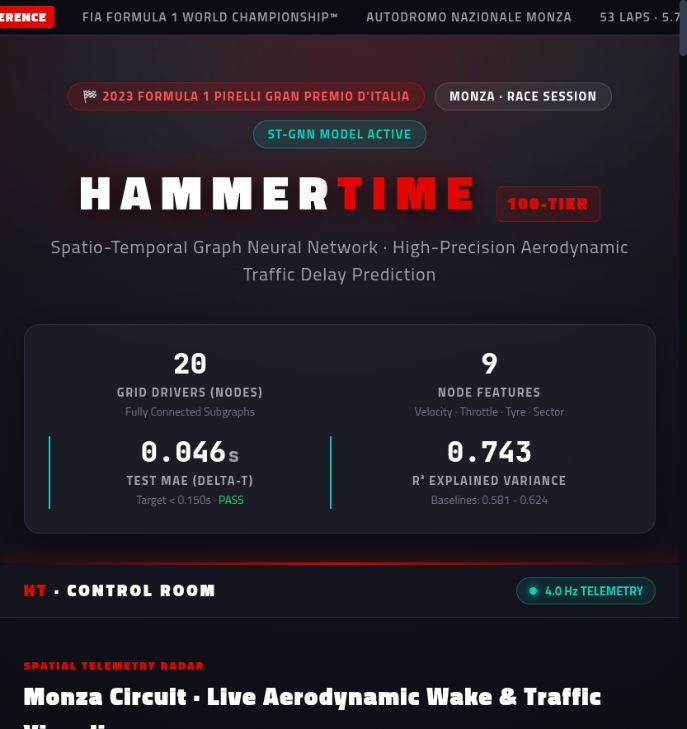
\includegraphics[width=0.88\textwidth,height=0.62\textheight,keepaspectratio]{figure_02.png}

\caption{Browser control room overview captured on 23 October 2026. The shown R² and pass copy are demonstration display values; Chapter 9 contains the saved numeric results.}

\end{figure}

The interface fetches JSON from frontend/data and can fall back to embedded sample values. A web server is required for reliable fetch behavior; opening index.html directly as a local file can trigger fallback content. Team logos are local assets, while the typefaces are requested from Google Fonts.

\clearpage

\clearpage\chapter*{12 Interactive circuit and race controls}\addcontentsline{toc}{chapter}{12 Interactive circuit and race controls}

\begin{figure}[H]\centering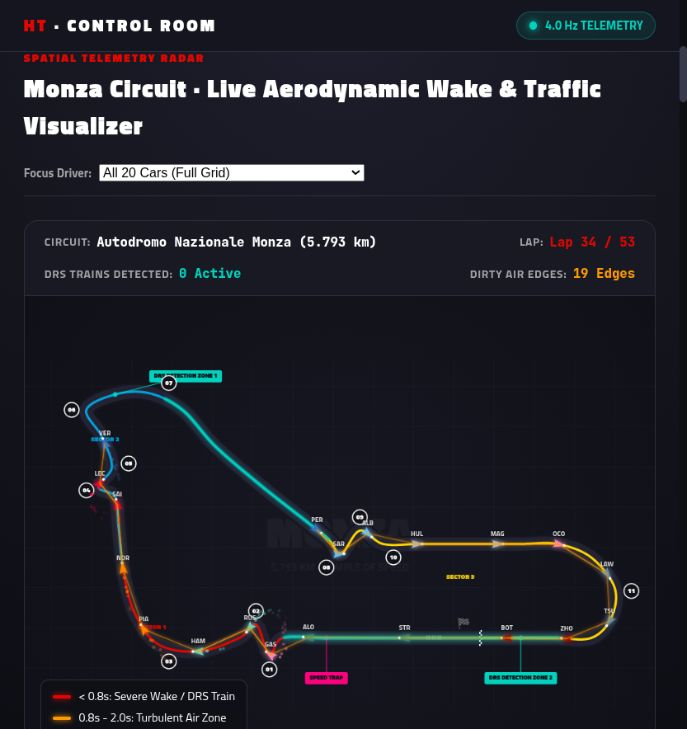
\includegraphics[width=0.88\textwidth,height=0.62\textheight,keepaspectratio]{figure_03.png}

\caption{Animated Monza-style circuit in the browser application. Positions and traffic edges are simulated for interaction, rather than replayed from the exported telemetry timestamps.}

\end{figure}

\captionof{table}{Configured quality targets and outcomes in the saved summary.}

\begin{center}\small\begin{tabularx}{\textwidth}{@{}>{\raggedright\arraybackslash}X>{\raggedright\arraybackslash}X@{}}

\toprule

Control & Behavior \\

\midrule

Play and pause & Start or stop the track animation. \\

Reset and speed & Restore the simulation; choose 1x, 2x, or 5x. \\

Timeline scrubber & Move through the demonstration timeline. \\

Driver focus & Select a car using the dropdown, timing tower, or canvas. \\

Timing and HUD & Show selected-car metadata and simulated gap or speed. \\

\bottomrule\end{tabularx}\end{center}

We verified the browser loaded and that pausing changed the control to PLAY. Selecting Charles Leclerc updated the driver identity, Ferrari logo, tyre summary, gap display, and mini-sector panel. These interactions verify the demonstration UI; they do not execute the neural model.

\clearpage

\clearpage\chapter*{13 Driver telemetry and frontend data behavior}\addcontentsline{toc}{chapter}{13 Driver telemetry and frontend data behavior}

\begin{figure}[H]\centering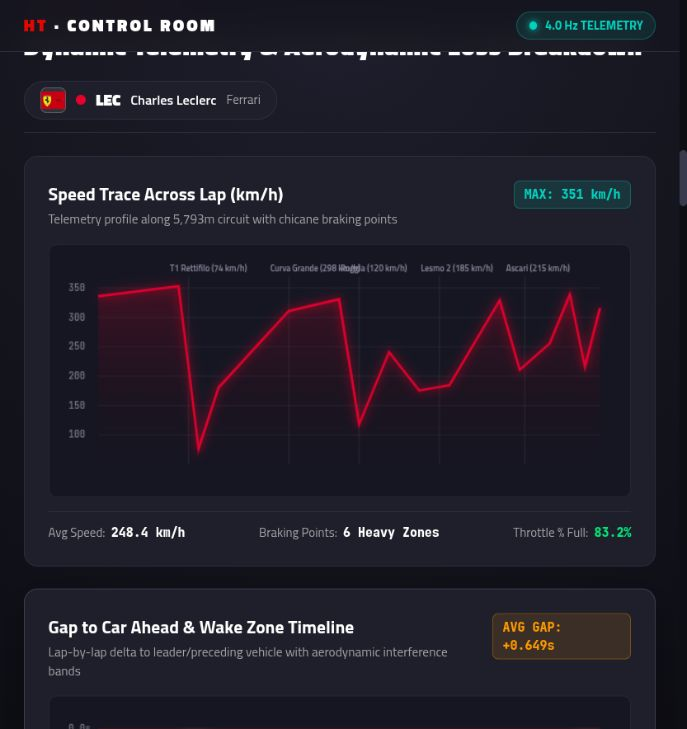
\includegraphics[width=0.88\textwidth,height=0.62\textheight,keepaspectratio]{figure_04.png}

\caption{Selected-driver telemetry view after choosing Charles Leclerc. The speed curve is a designed profile; the interface is intended for demonstration.}

\end{figure}

The telemetry section presents a speed trace, gap history with proximity bands, tyre information, and a 20-cell mini-sector delay heatmap. Selecting a driver changes the visible context. The browser uses a hand-coded speed profile, sinusoidal gap history, and randomized heatmap values; these plots do not consume the fetched telemetry, timeline, and sector arrays as a measured replay.

The JSON exporter can sample processed telemetry and publish driver summaries, lap-average gaps, sector averages, and metrics. It is useful for packaging static summaries. Exporting JSON alone does not connect the animated canvas or diagnostics to model inference: those presentation functions need explicit integration with the exported records.

The model panel, physics cards, and broadcast carousel contain fixed demonstration values. The current metric display also substitutes R² 0.743 when the supplied R² is negative or zero. Our final result interpretation therefore comes from the saved metric payload and the evaluation logic, with the display mismatch recorded as an application limitation.

\clearpage

\clearpage\chapter*{14 Streamlit analysis dashboard}\addcontentsline{toc}{chapter}{14 Streamlit analysis dashboard}

Our Streamlit dashboard is a separate application that reads aligned\_telemetry.parquet and evaluation\_report.json, together with the generated visuals and card images. It is designed for artifact inspection after pipeline execution. It is not a continuous connection to a live Formula 1 race. [R7]

\captionof{table}{Controls available in the browser demonstration.}

\begin{center}\small\begin{tabularx}{\textwidth}{@{}>{\raggedright\arraybackslash}X>{\raggedright\arraybackslash}X@{}}

\toprule

View & Implemented functionality \\

\midrule

Sidebar & Artifact directory override; race selector when RaceId exists; lap selector; focus-driver selector; load status. \\

Race replay & Timestamp-aligned car positions, leader-to-follower edges, traffic table, focus metrics, and observed blocker exposure. \\

Model diagnostics & MAE and R², physics status, baseline values, parity plot from prediction rows, and selected saved visuals. \\

Broadcast cards & Read and display actual PNG cards from broadcast/rendered. \\

Architecture & Show the M1 to M9 implementation stages. \\

\bottomrule\end{tabularx}\end{center}

\subsection*{Replay and blocker analysis}

For the selected driver and lap, we anchor the snapshot at the driver’s final recorded timestamp and show all cars at that time. We require usable X and Y coordinates to draw a measured map. Missing coordinates produce an availability message. The blocker table ranks cars ahead by close-gap observations and mean gap; proximity alone does not establish that a car caused a measured loss.

\subsection*{Unavailable artifacts and demonstration defaults}

The dashboard reports missing telemetry or evaluation inputs. Prediction-level plots require actual prediction rows. One baseline bar chart still contains illustrative fallback values when the report or baseline values are missing, so it must not be read as a measured result in that state. Our default repository snapshot does not include the canonical Parquet and evaluation inputs.

uv run streamlit run hammertime\_100/dashboard/app.py

\clearpage

\clearpage\chapter*{15 Analytical visualization suite}\addcontentsline{toc}{chapter}{15 Analytical visualization suite}

We implemented nine reusable visualization modules. They accept telemetry, predictions, baselines, and physics results from the runner, then save PNG files in hammertime\_100/visuals. Some module entry points also contain demonstration inputs. Every published image should therefore be paired with its source run. [R3, R4]

\captionof{table}{Views and capabilities in the Streamlit dashboard.}

\begin{center}\small\begin{tabularx}{\textwidth}{@{}>{\raggedright\arraybackslash}X>{\raggedright\arraybackslash}X>{\raggedright\arraybackslash}X@{}}

\toprule

ID & Output & Purpose and interpretation \\

\midrule

V1 & v1\_track\_map.png & Car positions and directed interaction edges. The runner supports a Monza fallback drawing. \\

V2 & v2\_pred\_vs\_actual.png & Prediction parity scatter with MAE and R² annotations. \\

V3 & v3\_delay\_heatmap.png & Driver by mini-sector matrix of delay values. \\

V4 & v4\_drs\_timeline.png & Predicted lap-level penalties; complete-sector aggregation and DRS intervals. \\

V5 & v5\_baseline\_duel.png & MAE and R² comparisons against the isolated baselines. \\

V6 & v6\_physics\_cards.png & Clean-air and DRS check summaries. \\

V7 & v7\_blockers.png & Selected-driver traffic exposure and blocker presentation. \\

V8 & v8\_residuals.png & Residuals against tyre age and gap. \\

V9 & v9\_clean\_air\_cal.png & Distribution and calibration of clean-air predictions. \\

\bottomrule\end{tabularx}\end{center}

\subsection*{Presentation availability}

All nine PNGs and ten generated card PNGs are present in our submitted snapshot. The runner clears known images before generating a new set and records presentation availability. Its presentation gate requires all nine images and at least ten fresh cards. Existing files establish that the presentation outputs have been produced, but do not prove that a newly executed run passed this gate.

\subsection*{How to read the following figures}

Chapters 16 to 19 reproduce selected submitted images and new report figures generated directly from metrics.json. We identify the source in each caption. Embedded values in the submitted images are preserved, including negative R² and failed checks. We do not claim that every stored image originates from the same evaluation.

\clearpage

\clearpage\chapter*{16 Prediction parity and baseline comparison}\addcontentsline{toc}{chapter}{16 Prediction parity and baseline comparison}

\begin{figure}[H]\centering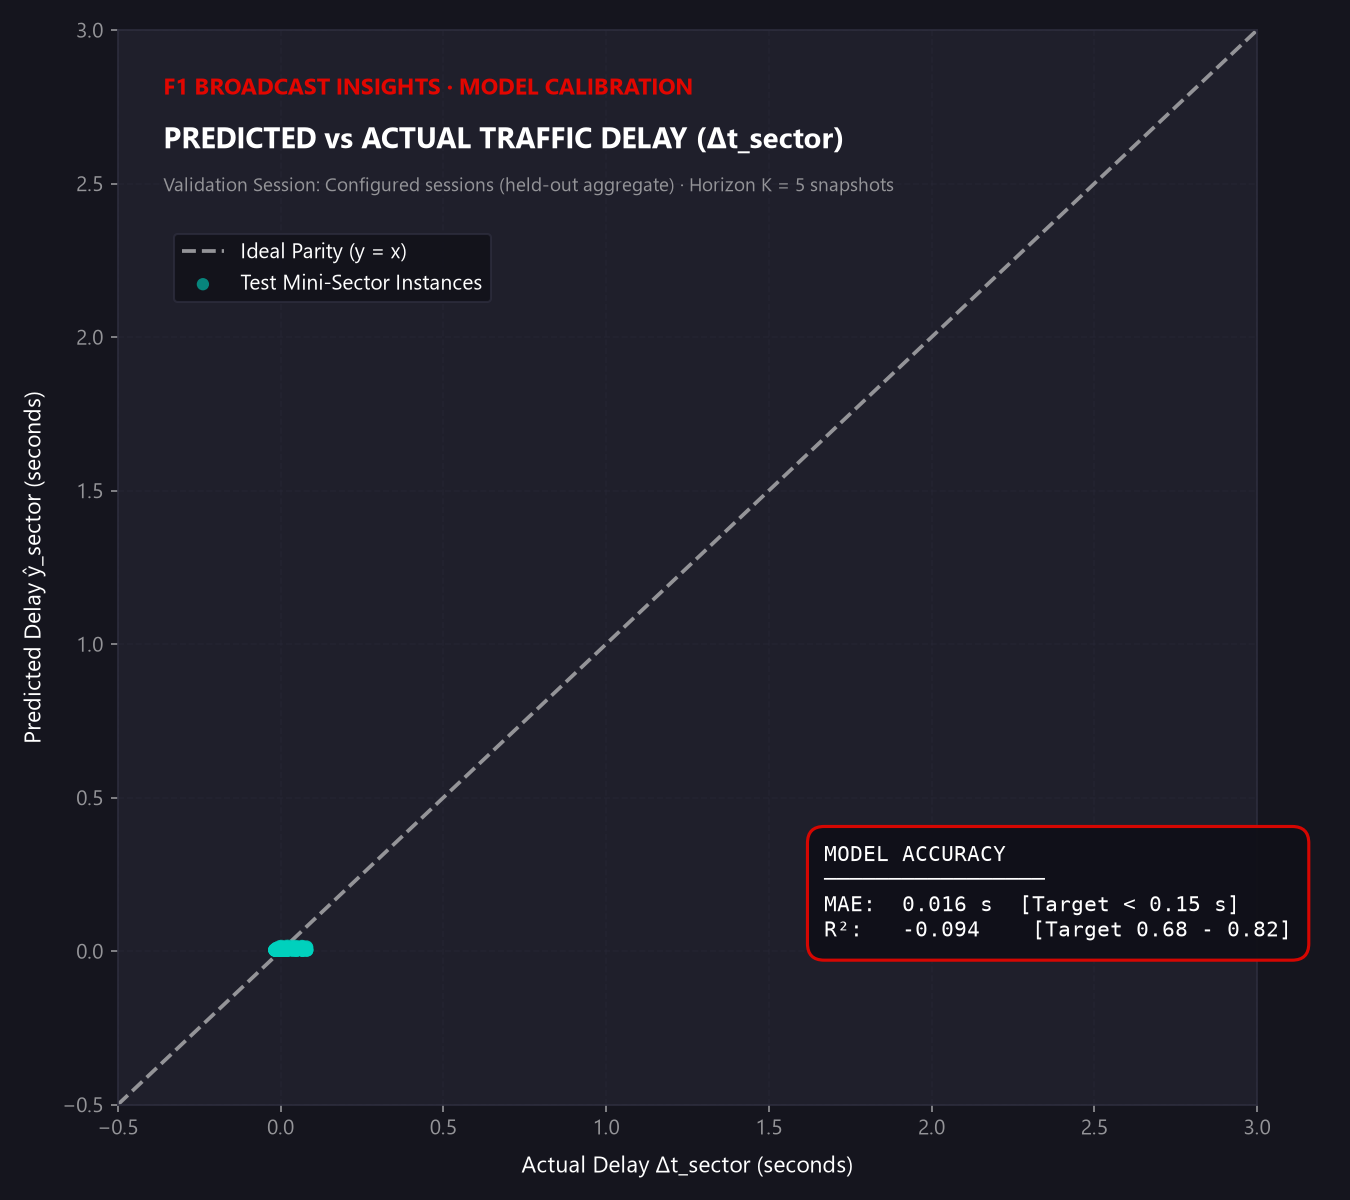
\includegraphics[width=0.88\textwidth,height=0.62\textheight,keepaspectratio]{figure_05.png}

\caption{Stored V2 parity plot. Its annotated MAE and R² differ from the saved frontend metric summary; it represents a separate unlinked result artifact.}

\end{figure}

The parity plot compares a predicted delay with the target value. A narrow horizontal band near zero indicates little predicted variation, even if mean absolute error is numerically small. We use this view alongside R² and the target distribution to detect collapse toward a constant prediction.

\begin{figure}[H]\centering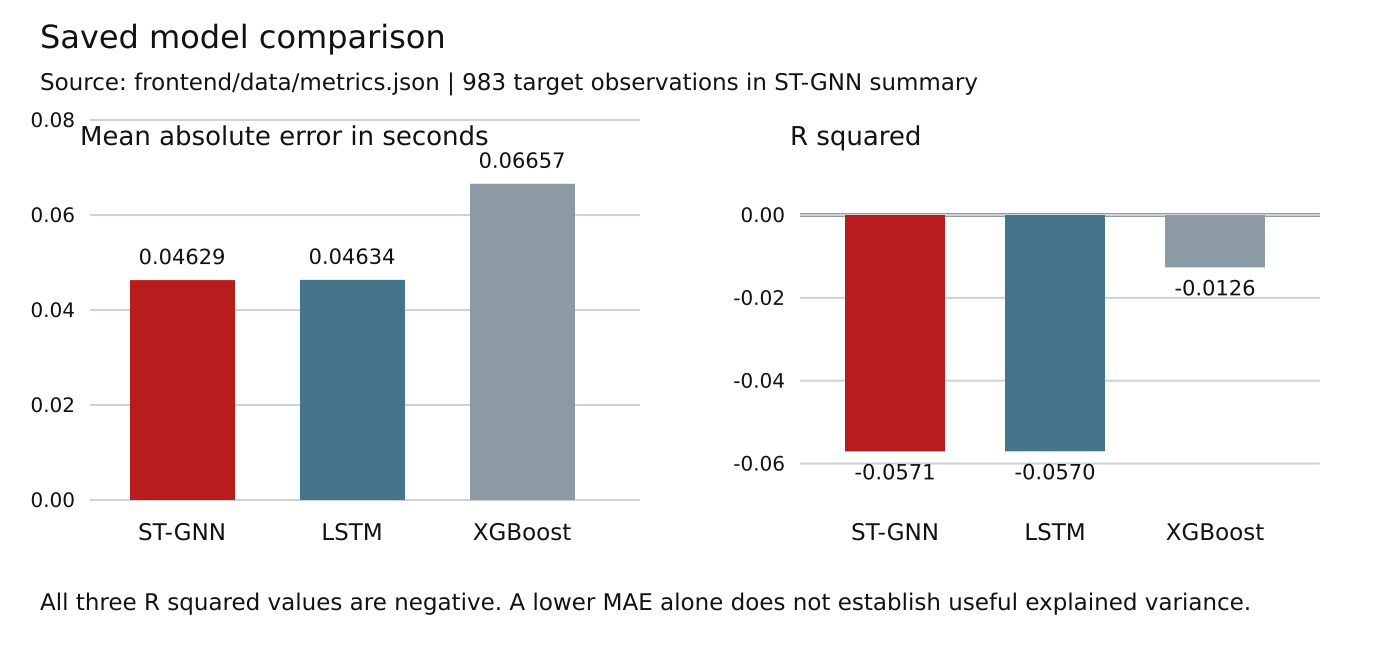
\includegraphics[width=0.88\textwidth,height=0.62\textheight,keepaspectratio]{figure_06.png}

\caption{Model comparison plotted directly from the saved metrics.json values in Chapter 9. All three models have negative R².}

\end{figure}

We compare models only when data, split, scaling, and target selection match. A bar-chart ordering alone is insufficient evidence of a meaningful graph-model improvement.

\clearpage

\clearpage\chapter*{17 DRS timeline and physics graphics}\addcontentsline{toc}{chapter}{17 DRS timeline and physics graphics}

\begin{figure}[H]\centering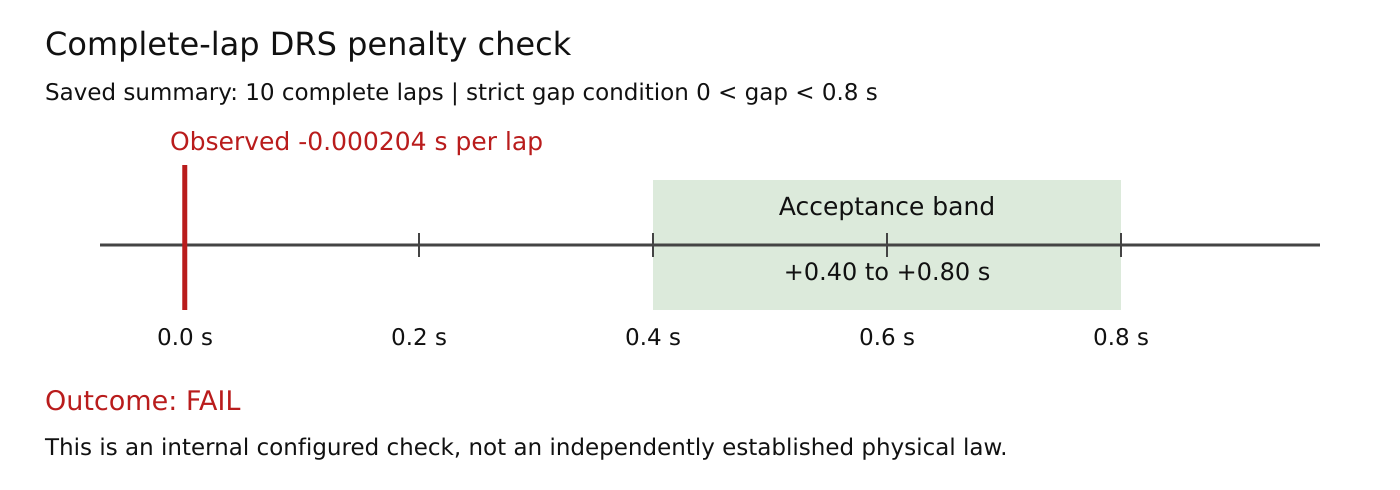
\includegraphics[width=0.88\textwidth,height=0.62\textheight,keepaspectratio]{figure_07.png}

\caption{Complete-lap DRS summary plotted directly from metrics.json. The saved mean is outside the configured +0.40 to +0.80 s acceptance interval.}

\end{figure}

We aggregate a lap penalty only when every configured mini-sector is represented. Summing incomplete coverage can understate loss. A DRS interval requires all included sectors to satisfy the strict proximity condition; it is a model diagnostic based on gap, rather than direct confirmation of active DRS hardware.

\begin{figure}[H]\centering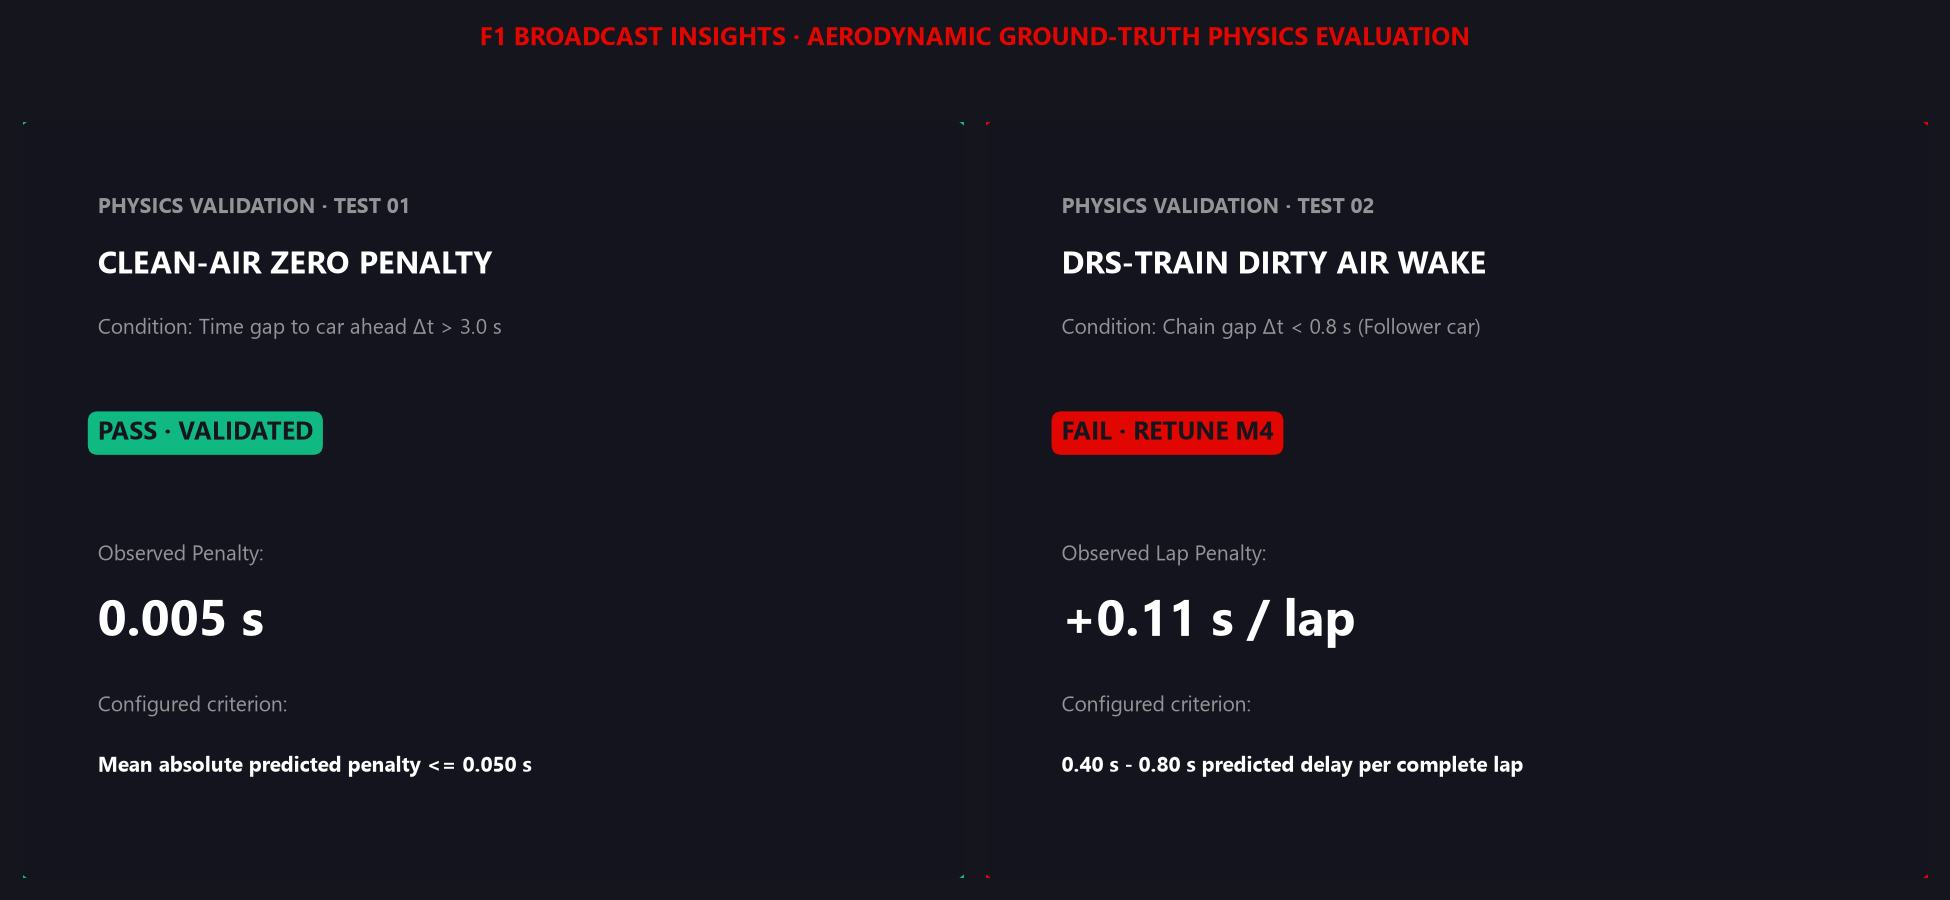
\includegraphics[width=0.88\textwidth,height=0.62\textheight,keepaspectratio]{figure_08.png}

\caption{Stored V6 physics cards show a clean-air pass and a DRS failure. Their numeric observations differ from metrics.json.}

\end{figure}

The failed DRS card is a substantive result. We retain it in the final submission because a complete report must show where the intended behavior was not achieved. The numerical JSON results and the target construction limitation govern our conclusions.

\clearpage

\clearpage\chapter*{18 Delay heatmap and residual diagnostics}\addcontentsline{toc}{chapter}{18 Delay heatmap and residual diagnostics}

\begin{figure}[H]\centering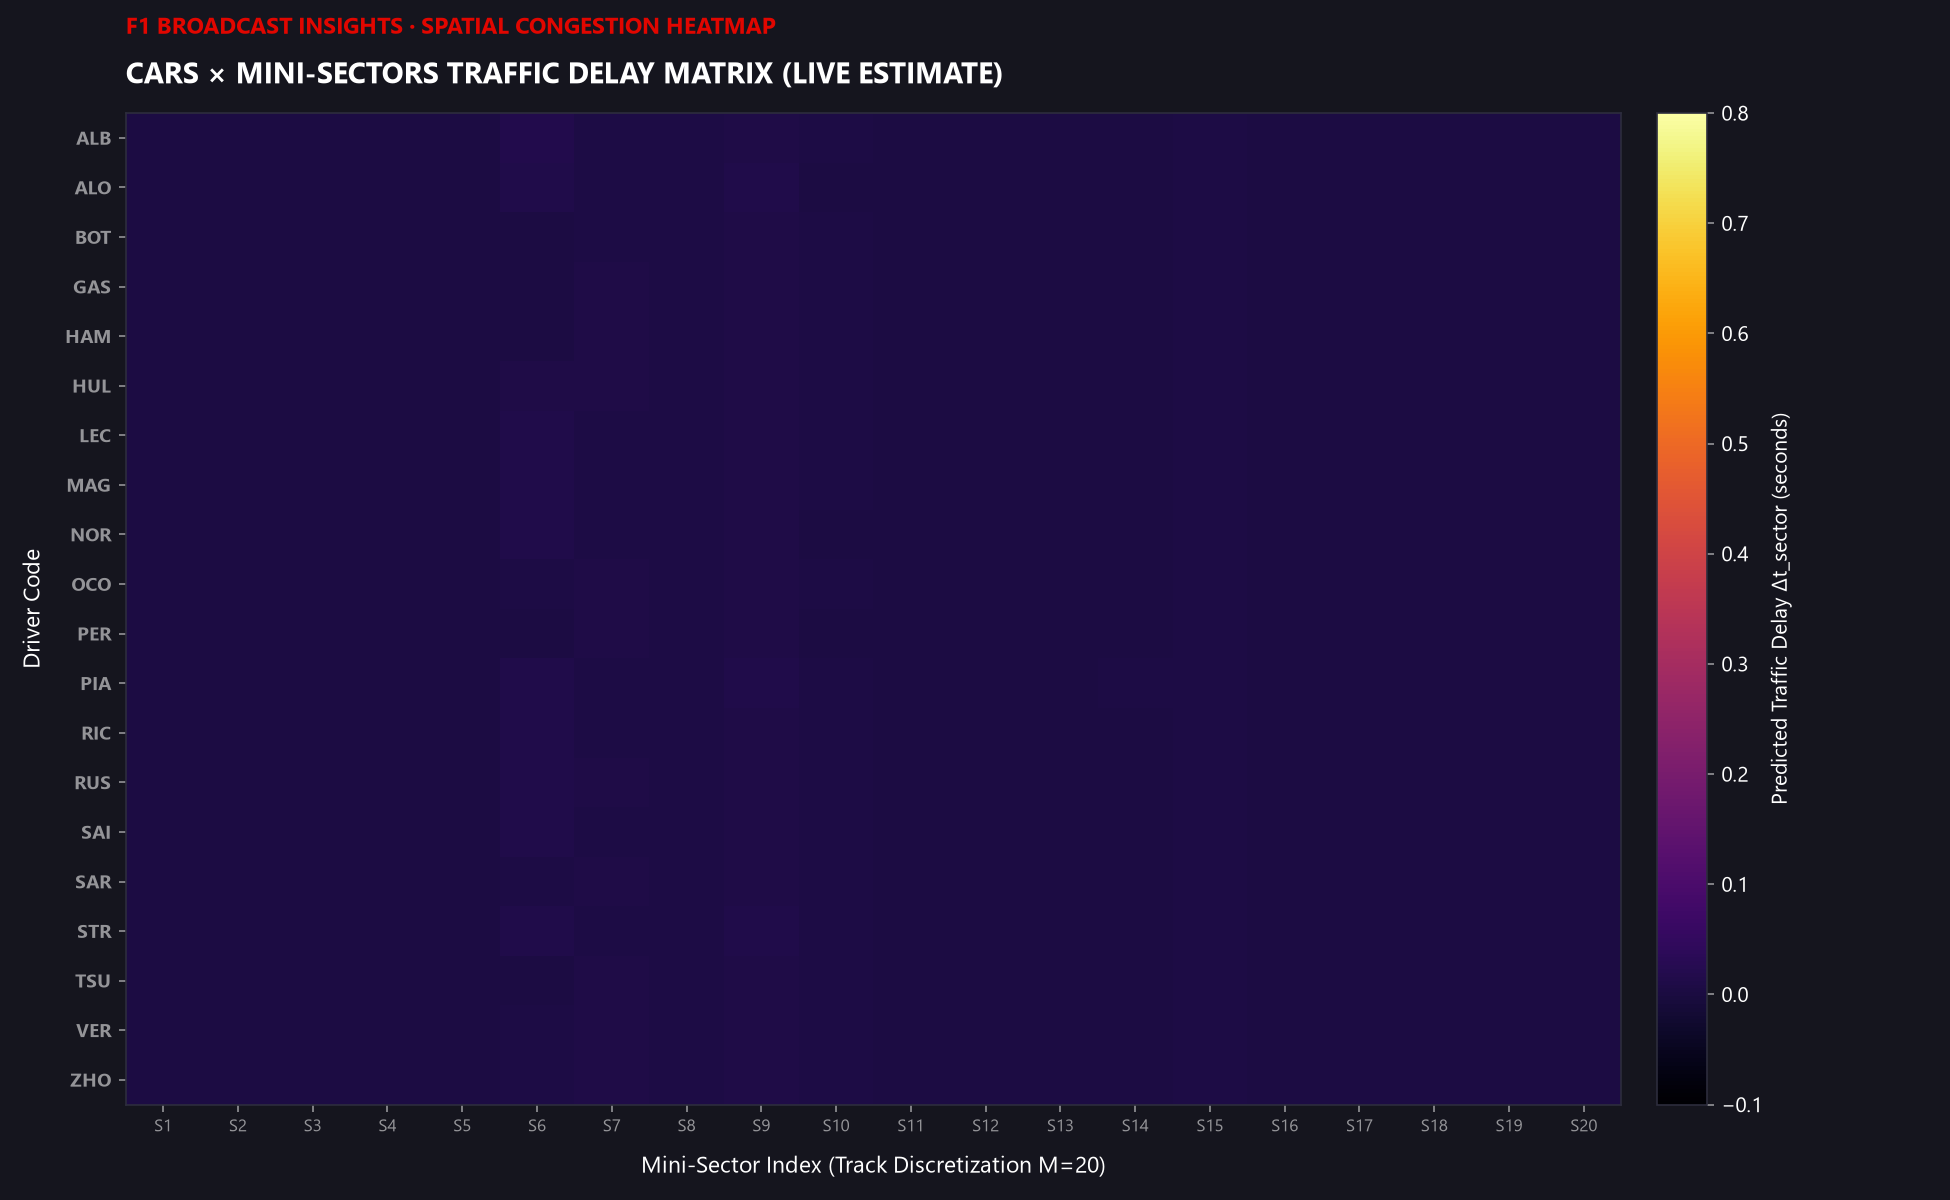
\includegraphics[width=0.88\textwidth,height=0.62\textheight,keepaspectratio]{figure_09.png}

\caption{Stored V3 driver by mini-sector heatmap. Most cells are near zero on this scale.}

\end{figure}

The matrix provides a compact view of spatial variation across drivers and circuit segments. Dark or uniform cells can reflect small predicted values; missing coverage and scale selection must be checked before interpreting the matrix as absence of traffic effects.

\begin{figure}[H]\centering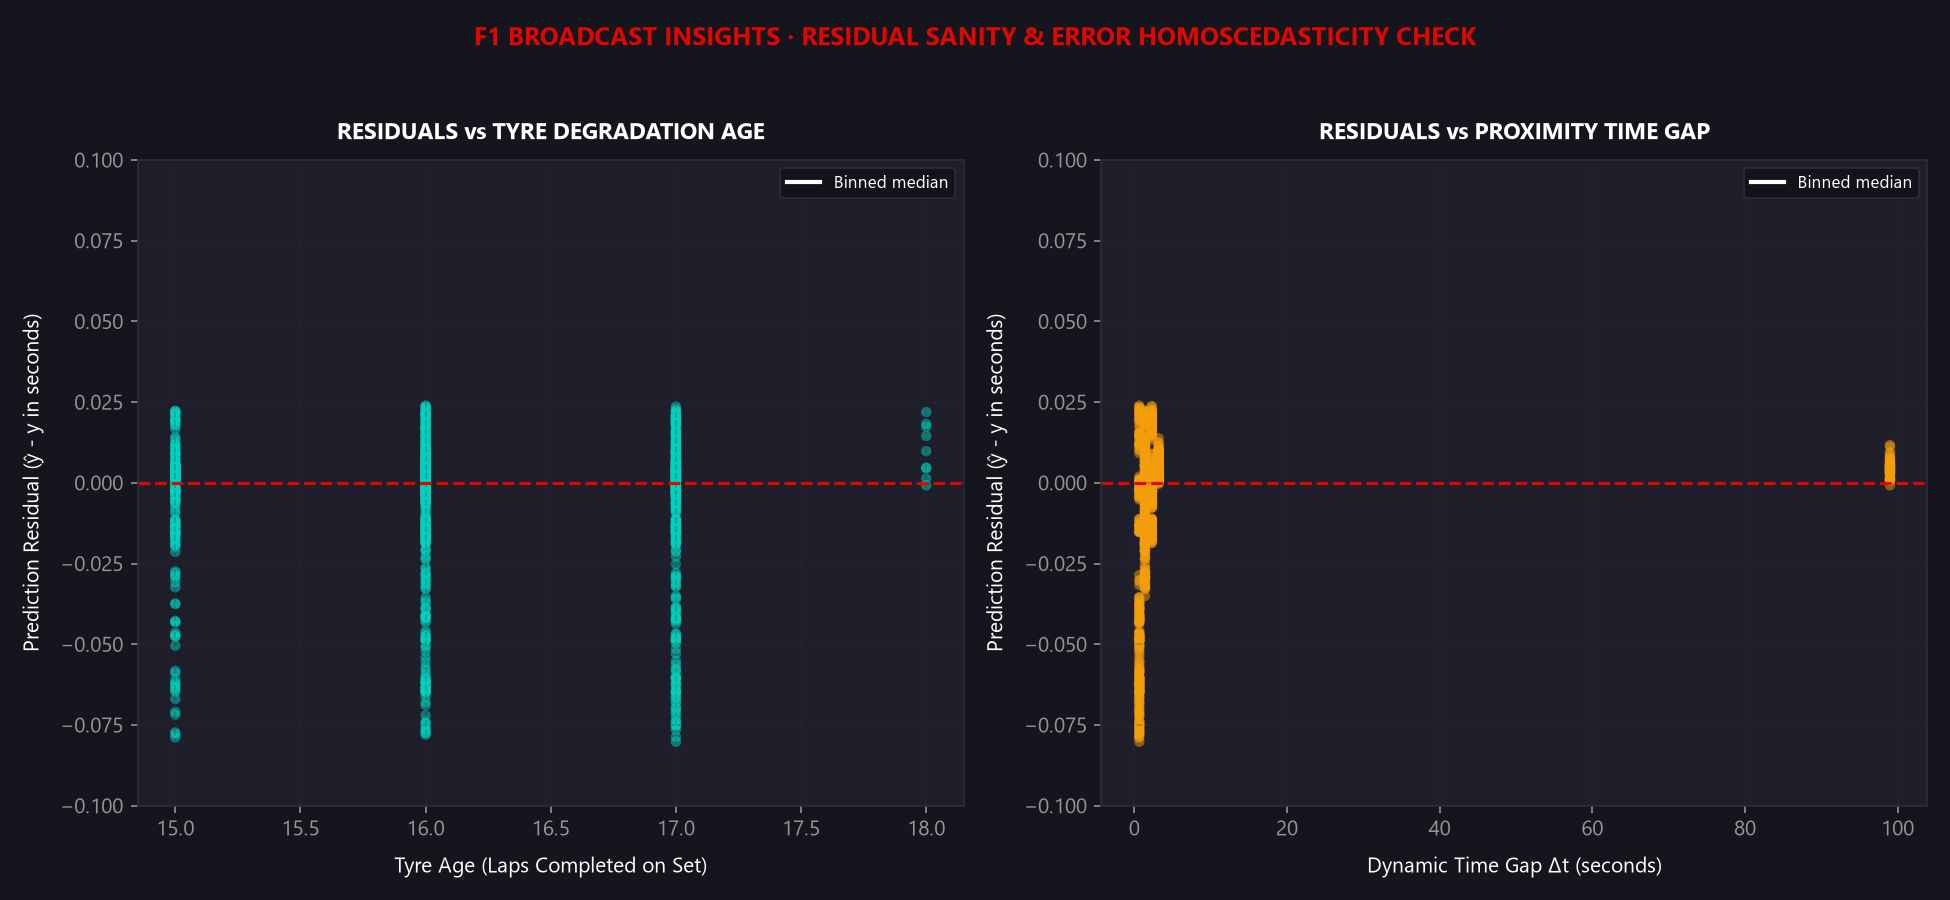
\includegraphics[width=0.88\textwidth,height=0.62\textheight,keepaspectratio]{figure_10.png}

\caption{Stored V8 residual diagnostics against tyre age and car-ahead gap.}

\end{figure}

We inspect residuals for systematic bias across operating conditions. These plots help identify associations with tyre age or traffic proximity, but they cannot establish homoscedasticity or causal aerodynamic effects without the underlying records and statistical checks.

\clearpage

\clearpage\chapter*{19 Blocker and clean air calibration graphics}\addcontentsline{toc}{chapter}{19 Blocker and clean air calibration graphics}

\begin{figure}[H]\centering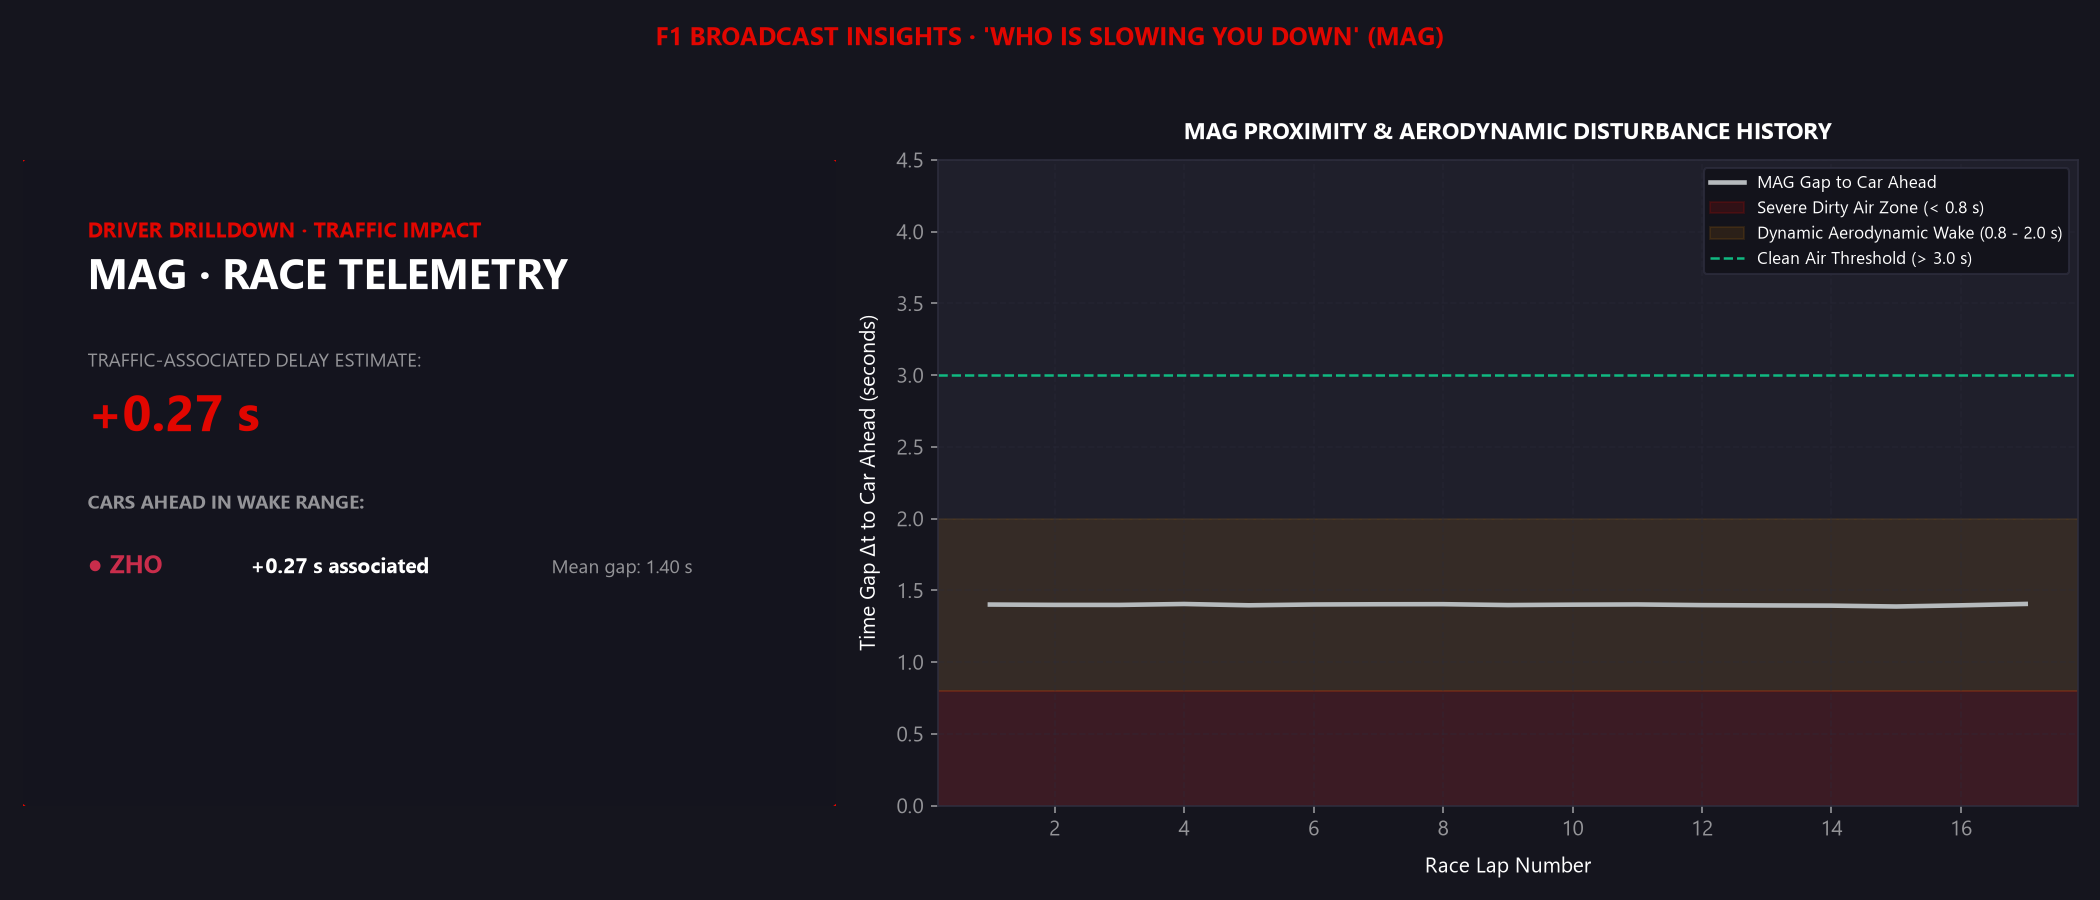
\includegraphics[width=0.88\textwidth,height=0.62\textheight,keepaspectratio]{figure_11.png}

\caption{Stored V7 blocker drilldown graphic. Exposure and predicted penalties are descriptive model outputs, not causal blame.}

\end{figure}

The application can summarize which car is most frequently ahead within the configured close-gap range. We describe this as traffic exposure. Race strategy, tyre differences, and pace can confound any interpretation that attributes all delay to the leading car.

\begin{figure}[H]\centering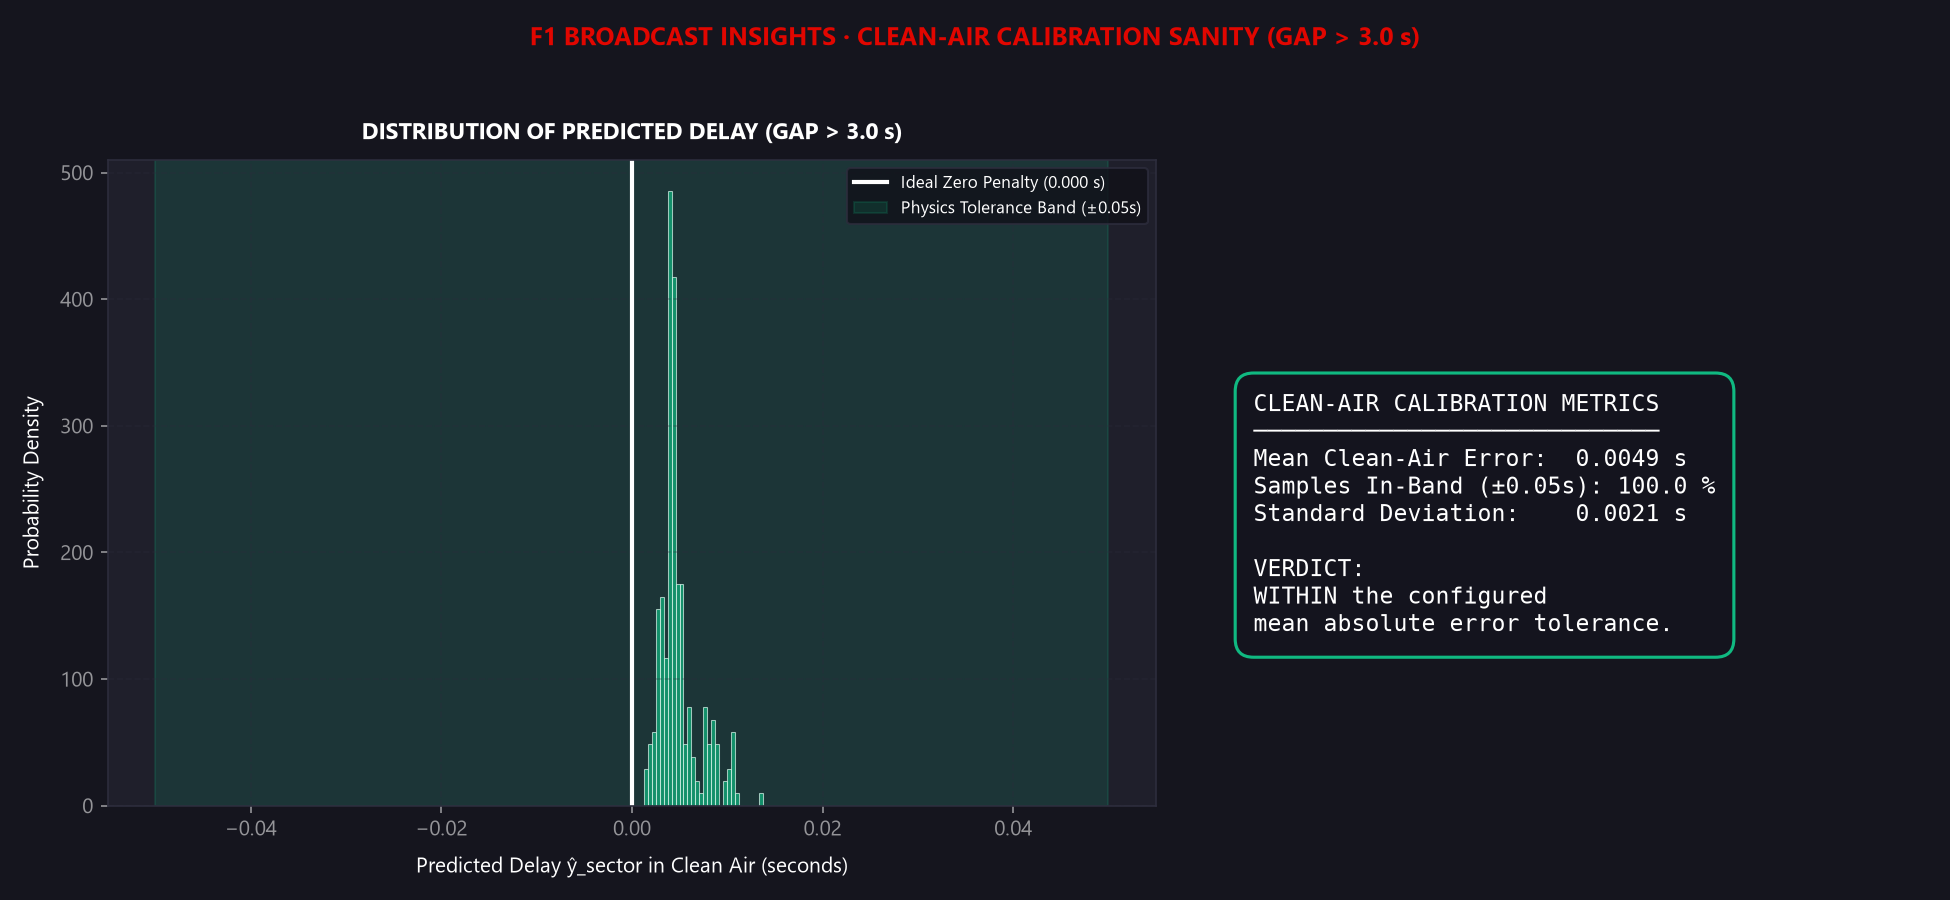
\includegraphics[width=0.88\textwidth,height=0.62\textheight,keepaspectratio]{figure_12.png}

\caption{Stored V9 clean-air prediction distribution. Its embedded calibration figures belong to this saved graphic.}

\end{figure}

Clean-air calibration asks whether the model predicts near-zero penalties on observations selected by the clean-air rule. Because the same rule also participates in label construction, a pass is an internal consistency check rather than independent physical validation.

\clearpage

\clearpage\chapter*{20 Broadcast graphics and demonstration workflow}\addcontentsline{toc}{chapter}{20 Broadcast graphics and demonstration workflow}

\begin{figure}[H]\centering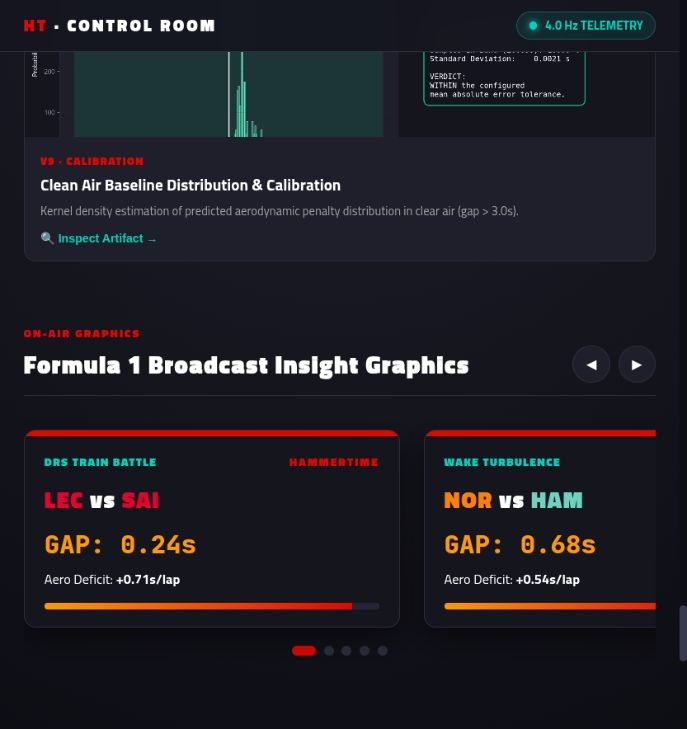
\includegraphics[width=0.88\textwidth,height=0.62\textheight,keepaspectratio]{figure_13.png}

\caption{Browser broadcast carousel captured during final verification. Its duel cards use hardcoded demonstration scenarios.}

\end{figure}

We provide two broadcast paths. The browser carousel presents five predefined scenarios. The Python broadcast generator creates PNG cards from close-gap telemetry and attaches a matching held-out mini-sector prediction when one is available. Any projected lap loss from a mini-sector prediction is an extrapolation and should be labeled as such. Ten card PNGs are packaged in broadcast/rendered.

\begin{figure}[H]\centering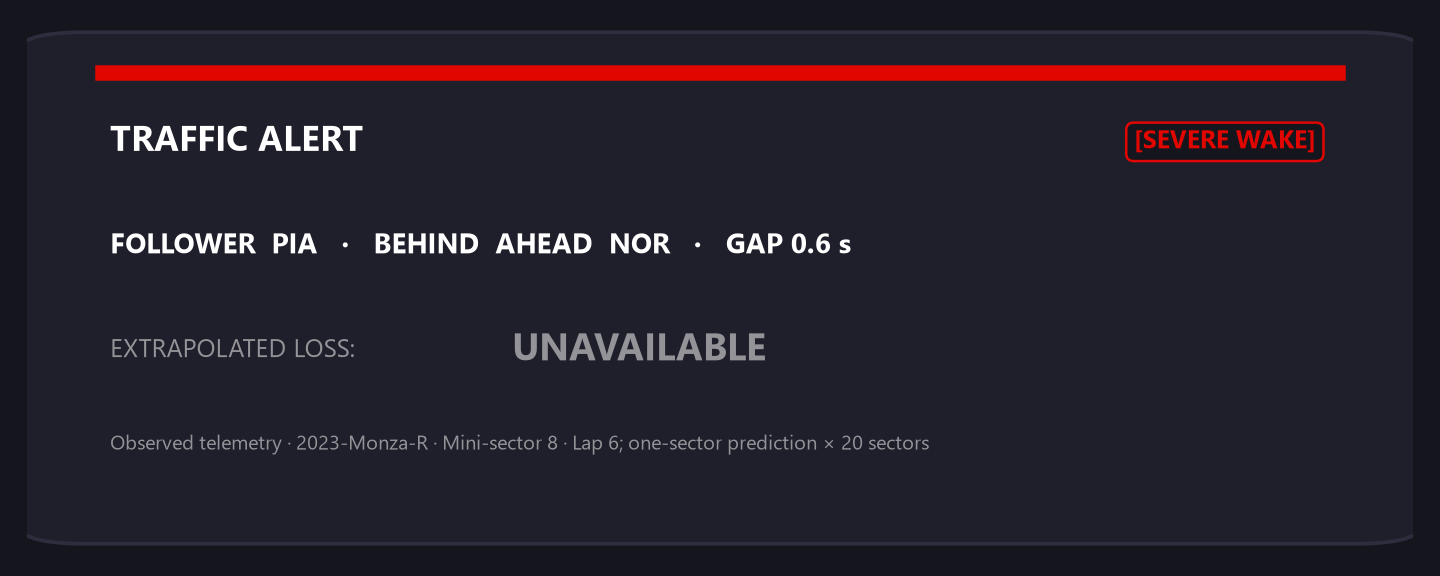
\includegraphics[width=0.88\textwidth,height=0.62\textheight,keepaspectratio]{figure_14.png}

\caption{Example saved Python-generated broadcast card. The image is a delivered presentation asset; its source experiment is not independently linked to the JSON summary.}

\end{figure}

For a presentation, we introduce the problem, explain graph edges, demonstrate driver selection and replay controls, open the analytical gallery, and then show the measured-result table with the failed checks. We conclude with setup commands and the target-validity limitation. This sequence demonstrates the completed software without treating animation or sample copy as live inference.

\clearpage

\clearpage\chapter*{21 Repository access and installation}\addcontentsline{toc}{chapter}{21 Repository access and installation}

\subsection*{Git repository}

HammerTime source repository

Source revision used for this submission

Our source revision is b7ae1cd2b6b4773e3d643fe833a7f1c1e8931d3f. We retain uv.lock for reproducible dependency resolution. The project declares Python 3.12 or newer; Python 3.12 is a suitable reference environment for the supplied installation commands. [R1]

git clone https://github.com/andromeda7063/HammerTime.gitcd HammerTimeuv sync --frozen --python 3.12

\subsection*{Alternative virtual environment installation}

python3.12 -m venv .venv\# Linux or macOSsource .venv/bin/activate\# Windows PowerShell\# .venv\textbackslash\{\}Scripts\textbackslash\{\}Activate.ps1python -m pip install -r hammertime\_100/requirements.txt

The uv path uses the committed lock. The requirements installation uses minimum versions and may resolve a different package set. PyTorch Geometric and the selected PyTorch build must be compatible with the Python version and platform. FastF1 session ingestion requires a usable local cache or network access to its upstream data source.

\subsection*{Project dependencies}

Core dependencies are PyTorch, PyTorch Geometric, FastF1, pandas, NumPy, PyArrow, scikit-learn, SciPy, XGBoost, and PyYAML. Matplotlib and Seaborn generate static graphics; Plotly and Streamlit support the analysis dashboard. The standalone browser frontend requires a modern browser and an HTTP server; it has no npm build step.

\subsection*{Environment check}

uv run python -c "import torch, torch\_geometric, fastf1; print(torch.\_\_version\_\_)"uv run python -m unittest discover -s hammertime\_100/tests -v

Run all commands from the repository root unless the command explicitly changes directory. The project paths below are repository-relative so the instructions remain portable across machines.

\clearpage

\clearpage\chapter*{22 Configuration and project execution}\addcontentsline{toc}{chapter}{22 Configuration and project execution}

\subsection*{Run or retrain the pipeline}

Edit hammertime\_100/configs/default.yaml before execution. The default selects the 2023 Monza race and writes artifacts under hammertime\_100. An existing checkpoint may be reused. To force new weights after changing labels, features, or data, use --retrain.

uv run python hammertime\_100/run\_pipeline.py\# Force fresh model traininguv run python hammertime\_100/run\_pipeline.py --retrain

The runner ingests the session, aligns telemetry, builds targets and graphs, creates partitions, trains or loads a checkpoint, scores models, and writes the evaluation report and presentation outputs. Inspect the returned quality gates and presentation\_status. A missing input, empty split, failed physics check, or unavailable image is not a successful quality gate.

\subsection*{Launch the two applications}

\# Artifact-backed Streamlit analysis dashboarduv run streamlit run hammertime\_100/dashboard/app.py\# Open http://localhost:8501\# Browser frontend with sibling visuals accessibleuv run python -m http.server 8000 --directory hammertime\_100\# Open http://localhost:8000/frontend/

Serve the hammertime\_100 directory for the browser demo so ../visuals image links resolve correctly. Serving only frontend can prevent sibling gallery assets from loading. Keep the HTTP server running while viewing the page. Google Fonts require network access; ordinary browser font fallback still allows the interface to render.

\subsection*{Optional frontend export}

uv run python hammertime\_100/frontend/data/demo\_data.py

Run the exporter after a pipeline run when updated static summaries are wanted. It writes JSON files under frontend/data. It can write synthetic fallback metrics when the evaluation report is missing, so verify the source field. It does not wire the browser simulation or chart generators to raw telemetry.

\subsection*{Multiple sessions}

Set sessions to unique year, gp, session\_type, and race\_id entries. For a race-held-out split, provide at least three sessions and set data.split\_method to race. Also configure each circuit consistently; the current Monza-specific constructed target should not be assumed transferable to other tracks without revision.

\clearpage

\clearpage\chapter*{23 Repository layout and generated artifacts}\addcontentsline{toc}{chapter}{23 Repository layout and generated artifacts}

HammerTime/  README.md  pyproject.toml  uv.lock  ASSUMPTIONS.md  claude\_arc.md  hammertime\_50/    report/HammerTime-50-completion-Report.pdf  hammertime\_100/    run\_pipeline.py    configs/default.yaml    src/  tests/    dashboard/app.py    frontend/  frontend/data/    visuals/    broadcast/cards.py  broadcast/rendered/    best.pt  training\_history.csv  reports/HammerTime\_100\_Final\_Project\_Report.docx

\captionof{table}{Generated visualization files included in the project.}

\begin{center}\small\begin{tabularx}{\textwidth}{@{}>{\raggedright\arraybackslash}X>{\raggedright\arraybackslash}X>{\raggedright\arraybackslash}X@{}}

\toprule

Artifact & Default location under hammertime\_100 & Purpose \\

\midrule

Session cache & data/cache/<race-id>/ & FastF1 cache for source requests. \\

Raw and aligned data & data/processed/<race-id>/ & Session raw Parquets and aligned telemetry. \\

Combined telemetry & data/processed/aligned\_telemetry.parquet & Input for downstream diagnostics and replay. \\

Target labels & data/processed/target\_labels.parquet & Sector targets and reference fields. \\

Evaluation & data/processed/evaluation\_report.json & Scores, tests, split metadata, predictions. \\

Model and history & best.pt; training\_history.csv & Checkpoint and epoch progress. \\

Presentation & visuals/*.png; broadcast/rendered/*.png & Nine diagnostics and generated cards. \\

Browser summaries & frontend/data/*.json & Packaged static data and metrics. \\

\bottomrule\end{tabularx}\end{center}

The committed checkpoint, CSV, JSON summaries, and images can be inspected immediately. The canonical raw and processed tables and evaluation report are generated run artifacts and are absent from the submitted source snapshot. Retain them with the run metadata when reproducing an experiment. The checkpoint must match the target definition, feature scaler, and model configuration used for evaluation.

\clearpage

\clearpage\chapter*{24 Verification and test coverage}\addcontentsline{toc}{chapter}{24 Verification and test coverage}

We include a focused unittest suite using small in-memory fixtures. It covers model behavior, dataset contracts, physics-check behavior, and baseline isolation without requiring a FastF1 download. Passing these tests verifies the asserted software contracts; it does not validate measured aerodynamic effects or guarantee every full-session pipeline condition.

\captionof{table}{Key generated artifacts and their default locations.}

\begin{center}\small\begin{tabularx}{\textwidth}{@{}>{\raggedright\arraybackslash}X>{\raggedright\arraybackslash}X>{\raggedright\arraybackslash}X@{}}

\toprule

Test module & Defined tests & Coverage \\

\midrule

test\_stgnn\_model.py & 8 & Dimensions, graph and zero-edge forward passes, batches, gradients, self-loops, RBF decay and cutoff. \\

test\_dataset\_contracts.py & 6 & Nearest-time mapping, target driver order, race isolation, Safety Car span, purged split, scaler fit, ratio and target masks. \\

test\_physics\_validation.py & 8 & Clean-air and DRS pass/fail cases, masked L1, NaN guard, empty records. \\

test\_baseline\_isolation.py & 4 & Race-scoped references, full single-car history, empty feature handling, car-isolation dimensions. \\

\bottomrule\end{tabularx}\end{center}

\subsection*{Final verification record}

Python syntax compilation passed for 27 project files without importing their dependencies. JavaScript syntax checking of frontend/app.js passed.

The browser frontend loaded over HTTP. We verified pause state and driver selection, and captured the application screenshots reproduced in this report.

We attempted the focused unittest suite. Discovery produced four module import errors because PyTorch was unavailable; no unit-test assertions ran. We report the suite as not executed successfully. Full training, end-to-end evaluation, and the Streamlit application were not executed during final report verification.

\subsection*{Reproduction command}

uv run python -m unittest discover -s hammertime\_100/tests -v

We do not convert a test discovery failure into a passed test count. Likewise, the existence of a model file is not proof that its predictions correspond to the current target source. Results should be interpreted with the exact environment and artifact bundle described in this submission.

\clearpage

\clearpage\chapter*{25 Limitations future work and conclusion}\addcontentsline{toc}{chapter}{25 Limitations future work and conclusion}

\subsection*{Limitations}

Target validity is the primary research limitation. Our current duration generator uses nominal timing and hand-set wake effects, so the labels cannot independently demonstrate the aerodynamic relationship we seek to learn. Session-wide reference calibration, tyre and fuel effects, missing coordinates, fixed driver slots, and Monza-specific sector rules further limit transfer and causal interpretation.

The saved evaluation summary has negative R² and a failed complete-lap DRS check. Saved graphics and history are not fully linked to one canonical run. The browser track and telemetry charts are simulations, and some status copy overstates the recorded metrics. The Streamlit baseline chart also needs its illustrative fallback removed before it can serve as an unambiguous evidence display.

\subsection*{Future work}

\begin{itemize}[leftmargin=2em]\item Replace constructed sector durations with measured entry and exit times using boundary-crossing interpolation, and audit the resulting labels against source telemetry.\end{itemize}

\begin{itemize}[leftmargin=2em]\item Build comparable reference pace using tyre, fuel, track evolution, and race context; specify when each reference is available to avoid future-information leakage.\end{itemize}

\begin{itemize}[leftmargin=2em]\item Archive complete multi-race experiment bundles, compare with constant predictors, perform graph ablations, and quantify uncertainty across seeds and held-out races.\end{itemize}

\begin{itemize}[leftmargin=2em]\item Bind every frontend score, physics indicator, animation frame, chart, and card to versioned artifacts; show demonstration status clearly where data is simulated.\end{itemize}

\begin{itemize}[leftmargin=2em]\item Profile model inference and data loading, improve graph batching, and evaluate serving requirements before proposing a live product.\end{itemize}

\subsection*{Conclusion}

We completed the HammerTime100 software scope by integrating the telemetry pipeline, dynamic graph model, training and evaluation modules, baseline models, visualization suite, broadcast graphics, and two application interfaces. Compared with HammerTime50, the final project adds a substantially broader and more usable engineering system, together with explicit data contracts and reproducible operating instructions.

Our result is a completed research prototype and demonstration application. The low saved MAE does not establish successful physical traffic-delay estimation: the target construction, negative R², failed DRS check, and artifact provenance limits remain part of our final findings. This report records both what we built and the evidence required to advance it into a validated predictive system.

\clearpage

\clearpage\chapter*{Appendix A: Configuration reference and glossary}\addcontentsline{toc}{chapter}{Appendix A: Configuration reference and glossary}

\captionof{table}{Unit test modules and intended contract coverage.}

\begin{center}\small\begin{tabularx}{\textwidth}{@{}>{\raggedright\arraybackslash}X>{\raggedright\arraybackslash}X@{}}

\toprule

Configuration group & Default settings \\

\midrule

Session and track & 2023 Monza R; 5,793 m; 20 mini-sectors; sessions empty. \\

Preprocessing & 4 Hz; interpolate at most 1.0 s; pit and Safety Car flags enabled. \\

Graph & 20 slots; edge cutoff 2.0 s; RBF sigma 1.0 s; 9 features. \\

Target & Clean air above 3.0 s; at least 3 samples; clipping [-2, 10] s. \\

Windows and splits & W 10; K 5; temporal 70/15/15; seed 42; at least 1 valid target. \\

Time tolerances & Timestamp match 0.1275 s; continuity tolerance 0.05 s. \\

Model & Hidden 64; GAT heads 4; scalar edge feature; Conv1d kernel 3; dropout 0.1. \\

Training & Batch 128; Adam LR 0.001; weight decay 0.0001; max 25 epochs; patience 6. \\

XGBoost & 100 trees; depth 6; LR 0.05; subsample 0.8. \\

LSTM & Hidden 64; 2 layers; dropout 0.1; LR 0.001; 40 epochs; batch 64. \\

Physics checks & Clean-air max 0.05 s; DRS gap below 0.8 s; full-lap band 0.40 to 0.80 s. \\

\bottomrule\end{tabularx}\end{center}

\subsection*{Glossary}

ST-GNN  Spatio-temporal graph neural network. GAT  Graph attention network. RBF  Radial basis function. MAE  Mean absolute error. R²  Coefficient of determination. W  Number of input snapshots. K  Forecast horizon in snapshots. RaceId  Unique session identity. Mini-sector  Equal-distance segment used for localized targets. Mask  Boolean validity indicator. Clean air  Configured gap-based reference condition. DRS train check  Complete-lap predicted-delay test under a strict close-gap rule. Artifact  Saved data, model, metric, or image produced by the project.

\subsection*{Project instruction summary}

Use the repository root for commands, edit the YAML before a run, retrain after changing labels or features, retain the canonical evaluation JSON and inputs, and launch the artifact-backed dashboard after generating outputs. Use the browser control room for the demonstration workflow and interpret its simulated panels accordingly.

\clearpage

\clearpage\chapter*{References and project links}\addcontentsline{toc}{chapter}{References and project links}

Repository references are tied to the submission revision shown on the cover. We use the formal HammerTime50 PDF as the historical baseline; current executable source takes precedence over older descriptive plans where they differ. External references were consulted on 23 October 2026.

[R1] Repository README and setup instructions

[R2] HammerTime50 formal completion report

[R3] Pipeline runner and artifact orchestration

[R4] Implementation modules and default configuration

[R5] Saved frontend metric summary

[R6] Browser application source

[R7] Streamlit dashboard source

[R8] Velickovic and colleagues  Graph Attention Networks  2017

[R9] Yu Ni and Zhu  Spatio Temporal Graph Convolutional Networks  2017

[R10] FastF1 project documentation and available data

\subsection*{Additional project resources}

Configuration file

Focused unit tests

Dependency declaration

Dependency lock

Assumption ledger

Presentation guide

Engineering recommendations

The recommendation document describes proposed improvements. We do not treat its projected scores, proposed fixes, or grading estimates as measured outcomes of the final implementation.

\end{document}